\documentclass[10pt]{article}
\usepackage[margin=1in]{geometry}
\usepackage{amsmath,amssymb,booktabs,graphicx,url,xcolor}
\usepackage[numbers,sort&compress]{natbib}
\usepackage{hyperref}

\title{The Anatomy of ``Beating PPO'': Exploration Walls, the Value Pathway,\\
and Where Model-Based Advantages Invert}
\author{Anonymous}
\date{}

\begin{document}
\maketitle

\begin{abstract}
Claims that model-based or structured methods ``beat PPO'' rarely survive matched-environment controls.
We run TD-MPC2, tuned brax PPO, and tuned brax SAC on byte-identical MJX environments and subject every
headline claim to an adversarial control. Three findings survive. (1)~\textbf{A categorical on-policy
exploration wall exists but is narrow}: on HopperHop, tuned PPO never reaches return 200 in 5/5 seeds at
472M steps, while SAC crosses by $\sim$8M and TD-MPC2 by $\sim$1M; on the same robot's easier Stand task the
wall is graded (PPO escapes 2/8; SAC solves 5/6 at 5M; TD-MPC2 3/3 by 0.9M), and five control tasks show no
wall at all. At a matched 1M budget, TD-MPC2 solves both hopper tasks while neither model-free method solves
either. (2)~\textbf{The mechanism is value learning, not dynamics modeling}: in a five-loss ablation replicated
at $n{\ge}4$ on three tasks, removing the TD value loss or the policy prior individually reproduces total
failure---including the exploration wall itself ($n{=}6$: the hop is never found)---while the reward head
matters only for planning and the self-predictive consistency loss is always the mildest cut.
(3)~\textbf{The advantage ordering is task-class-dependent and inverts on a 21-DoF humanoid}: TD-MPC2's
training diverges to NaN on 7/7 default-config runs (and its only numerically stable run never learns), PPO
is unusable under three configurations, and untuned SAC solves 4/5 --- on the high-DoF morphology only plain
off-policy learning works. We conclude that ``world model beats PPO'' decomposes into a sample-efficiency
and consistency advantage carried by the TD value pathway, real but confined to a characterizable dynamics
class, with no evidence of a level advantage anywhere.
\end{abstract}

\section{Introduction}
Model-based reinforcement learning methods such as TD-MPC2~\citep{hansen2024tdmpc2} report large advantages
over on-policy baselines like PPO~\citep{schulman2017ppo}. Such comparisons are sensitive to environment
mismatches, configuration errors, and seed-starved rate estimates. We present a case study in adversarial
self-review: every headline claim we initially formed was rewritten by its own control experiment, and we
report the final, control-surviving form together with the audit trail.

Our contributions:
\begin{itemize}
\item A matched-environment three-arm benchmark protocol (TD-MPC2 / tuned PPO / tuned SAC on byte-identical
MJX tasks), with two upstream configuration bugs found and documented by the audit (a task-name case mismatch
silently skipping tuned PPO hyperparameters; a missing humanoid configuration causing NaN under defaults).
\item A budget-indexed characterization of the on-policy exploration wall (Section~\ref{sec:wall}).
\item A five-loss ablation of TD-MPC2 replicated on three tasks at $n{\ge}4$ per arm, isolating the value
pathway as individually necessary (Section~\ref{sec:mech}).
\item A boundary result on a 21-DoF humanoid where the ordering inverts (Section~\ref{sec:boundary}).
\end{itemize}

\section{Setup}\label{sec:setup}
All methods interact with identical \texttt{mujoco\_playground} MJX environments
(\texttt{registry.load(env, impl=jax)}, episode length 1000, action repeat 1, verified byte-identical
across arms). PPO and SAC use the library's tuned configurations (2048 / 128 parallel environments); TD-MPC2
uses SimNorm latents with MPPI planning (2048 samples, horizon 3). Returns are best evaluation returns unless
stated. \emph{Config audit lesson:} the tuned-parameter lookup silently returns defaults on any name mismatch;
we audit resolved configurations for every run after discovering that \texttt{PendulumSwingUp} vs.\
\texttt{PendulumSwingup} voided the tuned override and manufactured a spurious ``wall.''

\section{The exploration wall, budget-indexed}\label{sec:wall}
\textbf{HopperHop --- categorical for PPO.} Tuned PPO: peak 53.8, 0/5 seeds ${\ge}200$ through 472M steps/seed;
the wall also survives the standard exploration knob (entropy cost $\times 3$ and $\times 10$: peaks 4--74,
$n{=}2$ each at 150M). On the \emph{graded} HopperStand barrier, by contrast, entropy $\times 3$ put 1/4 seeds over the threshold
(627 vs.\ 118--150; $\times 10$: 0/4, 116--185) --- a rate consistent with the baseline's 2/16 escape lottery
rather than a repair. The knob neither repairs the graded barrier nor dents the categorical wall.
SAC crosses 200 in 6/12 seeds by 5M and 6/9 by 8M (the 20M cohort crossed 5/5 at 4.1--7.7M; four direct-8M
seeds went 1/4 --- the crossing by 8M is a ${\sim}2/3$ rate, not a certainty). TD-MPC2: 6/6 by
${\sim}1$M; 5M bests 295--610, mean $420 \pm 113$ (sd, $n{=}12$).

\textbf{HopperStand --- graded but near-categorical.} PPO escapes 2/16 (eight further seeds at the full 285M
budget all walled at 105--195; both escapes, 681/749, peaked within 120M). SAC: 0/3 at 1M; 7/10 by 5M (solves
464--932; failures 33/100/300). TD-MPC2: 3/3 by ${\le}0.9$M (962/948/943; the third seed by 0.3M). The final
three-method gradient --- TD-MPC2 3/3 $\gg$ SAC 7/10 $\gg$ PPO 2/16 --- and the matched-1M column
(\emph{TD-MPC2 solves both hopper tasks at a budget where neither model-free method solves either}) are the
headline statements.

\begin{figure}[t]\centering
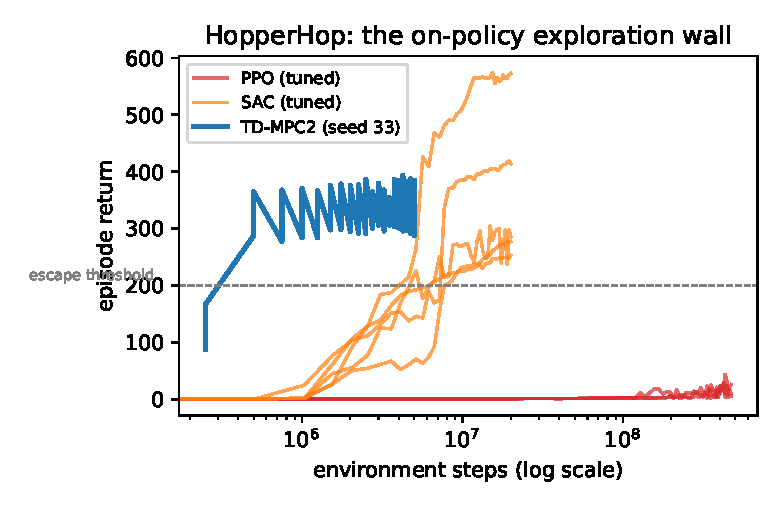
\includegraphics[width=0.62\linewidth]{figures/fig_wall_curves.pdf}
\caption{HopperHop seed curves on byte-identical MJX environments (log-$x$): tuned PPO stays below the escape
threshold through hundreds of millions of steps; tuned SAC crosses at 4--8M; TD-MPC2 crosses within 1M.}
\label{fig:wall}
\end{figure}

\textbf{No-wall controls.} FingerTurnHard (PPO ${\approx}973$, 3/3), Pendulum (solved once the config bug was
fixed: 842/831), BallInCupCatch (discovery-luck for both algorithms), CheetahRun (PPO 892--922 at 285M,
matching SAC 918/912 at 10M; an earlier ``never ${\ge}500$'' scoring was a budget/config artifact we retract),
WalkerRun. The wall is therefore specific to the single-leg hopper's unstable, contact-timing-critical
dynamics---categorical only for the hop itself.

\textbf{Discriminator: AcrobotSwingup (unstable, contact-free).} PPO learns normally (267--344, $n{=}4$ at
285M) --- \emph{the wall requires contact-criticality, not instability alone}. Conversely SAC is slow and
inconsistent here even at 20M (42/207; 54--89 at 5M): the off-policy advantage is also task-class-specific.
TD-MPC2 leads on both classes (429/422 within 1M) --- the value-pathway advantage is the most portable of the
three. (TD-MPC2 HopperStand later firmed to 5/5: 962/948/943/959/959.)

\section{Which loss does the work? The value pathway}\label{sec:mech}
We zero one loss term at a time (from scratch; masks verified in logs) and evaluate both MPPI and policy-only
returns, on CheetahRun, HopperHop, and WalkerRun, $n{\ge}4$ per decisive arm (HopperHop value cell $n{=}6$).

\begin{table}[h]\centering\small
\begin{tabular}{lllll}
\toprule
Arm & CheetahRun (MPPI best) & HopperHop & WalkerRun & Verdict\\
\midrule
full & 738/782/721/795 & 287--570 (6/6 find gait) & 699--723 & healthy\\
$-$value & 16/37/58 (dead) & \textbf{0.0/0.0/3.2/0.0/0.0/0.1 ($n{=}6$) --- gait never found} & 38--39 (dead) & \textbf{necessary}\\
$-$policy & MPPI limps 123--192; $\pi$ dead ${\le}11$ & ${\approx}0$ both readouts & 53--83 (dead) & \textbf{necessary}\\
$-$reward & MPPI 5--31; $\pi$ \textbf{761--805 (full)} & MPPI ${\approx}0$; $\pi$ 189--519 & MPPI 44; $\pi$ 681--728 (full) & planner-only\\
$-$consistency & 367--558 ($\pi$ to 623) & ${\sim}$half strength, 4/4 find gait & 483--674 & mildest\\
\bottomrule
\end{tabular}
\caption{Five-loss ablation. Removing the TD value loss reproduces the exploration wall itself; the
self-predictive dynamics loss is the only component whose removal merely degrades.}
\end{table}

\begin{figure}[t]\centering
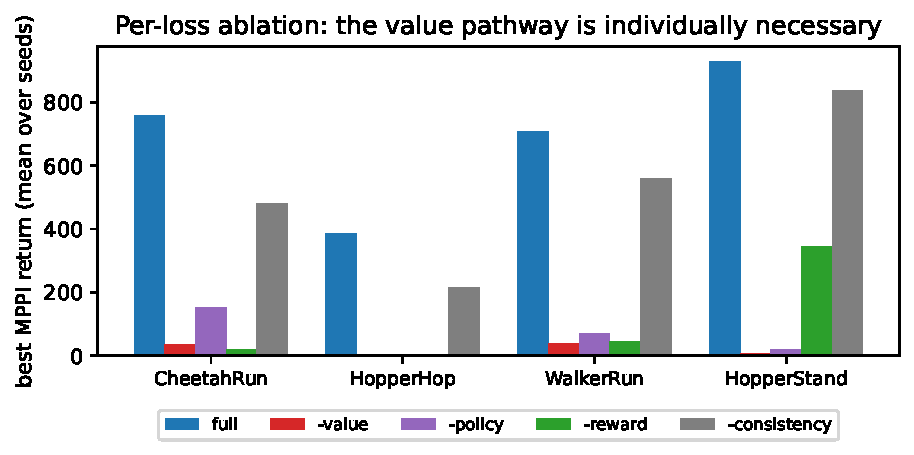
\includegraphics[width=0.8\linewidth]{figures/fig_mechanism_bars.pdf}
\caption{Five-loss ablation across four tasks (best MPPI return, mean over seeds, $n{\ge}2$ per bar; decisive
arms $n{\ge}4$). Removing the TD value loss or the policy prior is fatal everywhere; removing the
self-predictive consistency loss barely registers.}
\label{fig:mech}
\end{figure}

The pattern replicates on a fourth task, HopperStand ($n{=}4$/arm), which the full model solves in 0.3M steps:
none 911--946 (all solve); value-ablated 6--13 and policy-ablated 9--34 --- dead; reward-ablated MPPI 265--542
but $\pi$ 943--944; consistency-ablated 816--898 --- nearly no cut at all. \emph{Without the TD value loss,
TD-MPC2 cannot even learn to stand.}

The ablation's mildest cut is not uniformly removable, and the pattern is sharper than a task-class split.
Training consistency-OFF from scratch at the full 5M budget: on HopperHop the stripped agent scores
165/475/481/511 ($n{=}4$) against the full model's $420 \pm 113$ ($n{=}12$) --- three seeds at the top of the
full band, reaching 440+ by ${\sim}2$M --- but on every other task tested the stripped agent loses badly:
WalkerRun 537--594 (mean 565) vs.\ 709--782 (mean 737), $-23\%$; CheetahRun 516--528 (mean 524) vs.\ 782--904
(mean 849), $-38\%$; AcrobotSwingup 233--352 (mean 284) vs.\ 488--533 (mean 511), $-44\%$ --- all
non-overlapping ($n{=}4$ per cell). Acrobot is exploration-flavored, so ``removable when exploration-bound''
does not survive; the reading that fits all four tasks is that the self-predictive loss underwrites MPPI
rollout quality wherever the \emph{planner} carries learning, and HopperHop --- where the policy head learns
the behavior directly --- is the one task where it is redundant.

``The world model explores'' thus decomposes: the TD value signal trained through the latent discovers and
ranks behavior; the self-predictive dynamics loss is a helpful regularizer, not the key.

\section{Level vs.\ efficiency; hierarchy control}\label{sec:level}
At 4$\times$ TD-MPC2's budget (20M), SAC finals on HopperHop are 246/277/285/414/572 ($n{=}5$) --- the
distributions overlap TD-MPC2's ${\sim}$412--481. The world model's robust advantages are \emph{consistency}
and ${\sim}$4--5$\times$ sample-efficiency, not a level ceiling. A dense-shaping control also re-attributes a
feudal-hierarchy ``win'' (4/6 vs.\ flat 0/6) to signal density: shaped flat TD3 solves 3/6; the surviving
claim is that the hierarchy \emph{self-generates} that signal (replicating~\citealp{nachum2019hrl}).

\section{The boundary: a 21-DoF humanoid inverts the ordering}\label{sec:boundary}
On DMC HumanoidWalk: PPO produces \texttt{reward=nan} under all three configurations tried (no official tuned
humanoid configuration exists upstream). TD-MPC2's training loss diverges to NaN on 6/6 default-config walk
seeds (onsets 0.53--2.51M) and on the easier Stand (0.28M); best return before any divergence was 30.4.
Reducing the update-to-data ratio shifts the onset stochastically ($k{=}32$: NaN at 3.13M; $k{=}64$: the only
run of nine to finish 4M) --- and the surviving run never learns (best 21.8). Untuned SAC solves 4/5
(625--909 at 5M; 1/5 NaN). Config/numerical robustness is thus a failure axis orthogonal to exploration, and
any ``X beats PPO'' claim must state which axis it lives on.

\section{Related work}\label{sec:related}
Sample-efficiency victories for model-based and hybrid methods are well replicated
(EfficientZero~\citep{ye2021efficientzero}, DreamerV3~\citep{hafner2023dreamerv3},
TD-MPC2~\citep{hansen2024tdmpc2}, RLPD~\citep{ball2023rlpd}); asymptotic-level victories keep eroding as
model-free baselines are scaled and regularized (BRO~\citep{nauman2024bro}, SimBa~\citep{lee2024simba},
TD7~\citep{fujimoto2023td7}, CrossQ~\citep{bhatt2024crossq}); most measurable HRL benefit reproduces on flat
agents given better exploration/shaping~\citep{nachum2019hrl}. Our results agree from an independent,
matched-environment direction and add the per-loss attribution and the high-DoF inversion.

\section{Discussion}\label{sec:discussion}
Every one of our initial headline claims (``gait-specific wall,'' ``morphology-categorical wall,'' ``world
model buys level,'' ``hierarchy beats flat'') died under one more seed or one more control, always toward a
smaller, truer statement. The surviving picture: structured priors and world models buy speed and
consistency, never ceiling; their engine is value learning; and their advantage region is a characterizable
dynamics class outside of which the ordering can fully invert. We offer the audit trail (public ledger and
blog) as a template for adversarial self-review.

\bibliographystyle{plainnat}
\begin{thebibliography}{20}
\bibitem[Ball et al.(2023)]{ball2023rlpd} P.~Ball et al. Efficient online RL with offline data. ICML 2023.
\bibitem[Bhatt et al.(2024)]{bhatt2024crossq} A.~Bhatt et al. CrossQ. ICLR 2024.
\bibitem[Fujimoto et al.(2023)]{fujimoto2023td7} S.~Fujimoto et al. For SALE: state-action representation learning. NeurIPS 2023.
\bibitem[Hafner et al.(2023)]{hafner2023dreamerv3} D.~Hafner et al. Mastering diverse domains through world models. arXiv:2301.04104.
\bibitem[Hansen et al.(2024)]{hansen2024tdmpc2} N.~Hansen, H.~Su, X.~Wang. TD-MPC2. ICLR 2024.
\bibitem[Lee et al.(2024)]{lee2024simba} H.~Lee et al. SimBa. arXiv:2410.09754.
\bibitem[Nachum et al.(2019)]{nachum2019hrl} O.~Nachum et al. Why does hierarchy (sometimes) work so well in RL? arXiv:1909.10618.
\bibitem[Nauman et al.(2024)]{nauman2024bro} M.~Nauman et al. Bigger, regularized, optimistic (BRO). NeurIPS 2024.
\bibitem[Schulman et al.(2017)]{schulman2017ppo} J.~Schulman et al. Proximal policy optimization. arXiv:1707.06347.
\bibitem[Ye et al.(2021)]{ye2021efficientzero} W.~Ye et al. Mastering Atari games with limited data. NeurIPS 2021.
\end{thebibliography}

\end{document}
